\begin{figure}[H]
  \centering
  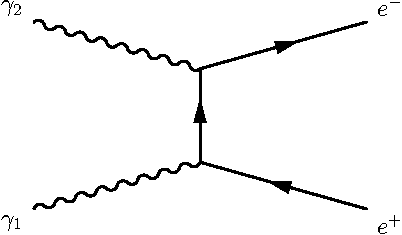
\includegraphics{feynmp/yy_ee.pdf}
\end{figure}

\begin{equation}
  P_1 + P_2 = P_{+} + P_{-}
\end{equation}
After squaring both sides, since $m_1=m_2=0$,
\begin{equation}
  2E_1E_2 = 4m_e^2 \quad \Rightarrow \quad E_1 = \frac{2m_e^2}{E_2}.
\end{equation}
%
For $\lambda_2 = \SI{1}{\micro\meter}$,
\begin{equation}
  E_2 = \frac{hc}{\lambda} = 1.24\eV
\end{equation}
\begin{equation}
  E_1 = \frac{2\times (0.511\times 10^6)^2}{1.24} \eV
      = 4.2\times 10^{11} \eV = \boxed{ 0.42 \TeV }
\end{equation}


